%-------------------------------------------------------------------------------------------------------------------------------------------------------------------------------------------------
% Section 2
%
%-------------------------------------------------------------------------------------------------------------------------------------------------------------------------------------------------
\section{Line ensembles}\label{Section2}
In this section we introduce various definitions and notation that are used throughout the paper. 

%-------------------------------------------------------------------------------------------------------------------------------------------------------------------------------------------------
% Section 2.1
%
%-------------------------------------------------------------------------------------------------------------------------------------------------------------------------------------------------
\subsection{Line ensembles and the Brownian Gibbs property}\label{Section2.1}
In this section we introduce the notions of a {\em line ensemble} and the {\em (partial) Brownian Gibbs property}. Our exposition in this section closely follows that of \cite[Section 2]{DimMat} and \cite[Section 2]{CorHamA}. 

Given two integers $p \leq q$, we let $\llbracket p, q \rrbracket$ denote the set $\{p, p+1, \dots, q\}$. Given an interval $\Lambda \subset \mathbb{R}$ we endow it with the subspace topology of the usual topology on $\mathbb{R}$. We let $(C(\Lambda), \mathcal{C})$ denote the space of continuous functions $f: \Lambda \rightarrow \mathbb{R}$ with the topology of uniform convergence over compacts, see \cite[Chapter 7, Section 46]{Munkres}, and Borel $\sigma$-algebra $\mathcal{C}$. Given a set $\Sigma \subset \mathbb{Z}$ we endow it with the discrete topology and denote by $\Sigma \times \Lambda$ the set of all pairs $(i,x)$ with $i \in \Sigma$ and $x \in \Lambda$ with the product topology. We also denote by $\left(C (\Sigma \times \Lambda), \mathcal{C}_{\Sigma}\right)$ the space of continuous functions on $\Sigma \times \Lambda$ with the topology of uniform convergence over compact sets and Borel $\sigma$-algebra $\mathcal{C}_{\Sigma}$. Typically, we will take $\Sigma = \llbracket 1, N \rrbracket$ (we use the convention $\Sigma = \mathbb{N}$ if $N = \infty$) and then we write  $\left(C (\Sigma \times \Lambda), \mathcal{C}_{|\Sigma|}\right)$ in place of $\left(C (\Sigma \times \Lambda), \mathcal{C}_{\Sigma}\right)$.




The following defines the notion of a line ensemble.
\begin{definition}\label{CLEDef}
Let $\Sigma \subset \mathbb{Z}$ and $\Lambda \subset \mathbb{R}$ be an interval. A {\em $\Sigma$-indexed line ensemble $\mathcal{L}$} is a random variable defined on a probability space $(\Omega, \mathcal{F}, \mathbb{P})$ that takes values in $\left(C (\Sigma \times \Lambda), \mathcal{C}_{\Sigma}\right)$. Intuitively, $\mathcal{L}$ is a collection of random continuous curves (sometimes referred to as {\em lines}), indexed by $\Sigma$,  each of which maps $\Lambda$ in $\mathbb{R}$. We will often slightly abuse notation and write $\mathcal{L}: \Sigma \times \Lambda \rightarrow \mathbb{R}$, even though it is not $\mathcal{L}$ which is such a function, but $\mathcal{L}(\omega)$ for every $\omega \in \Omega$. For $i \in \Sigma$ we write $\mathcal{L}_i(\omega) = (\mathcal{L}(\omega))(i, \cdot)$ for the curve of index $i$ and note that the latter is a map $\mathcal{L}_i: \Omega \rightarrow C(\Lambda)$, which is $(\mathcal{C}, \mathcal{F})-$measurable.
\end{definition}

We will require the following result, whose proof is postponed until Section [Appendix]. In simple terms it states that the space $C (\Sigma \times \Lambda)$ where our random variables $\mathcal{L}$ take value has the structure of a complete, separable metric space. We say that a collection $(K_n)_{n\geq 1}$ of compact subsets $K_n\subset\Sigma\times\Lambda$ is a \textit{compact exhaustion} if $K_n\subseteq K_{n+1}$ for all $n\geq 1$, $\bigcup_n K_n = \Sigma\times\Lambda$, and every compact subset of $\Sigma\times\Lambda$ is contained in some $K_n$.
\begin{lemma}\label{Polish} Let $(K_n)_{n\geq 1}$ be a compact exhaustion of $\Sigma\times\Lambda$. Define $d: C (\Sigma \times \Lambda) \times C (\Sigma \times \Lambda) \rightarrow [0, \infty)$ by
\begin{equation} d (f,g) = \sum_{n=1}^\infty 2^{-n}\min\Big\{\sup_{(i,t)\in K_n} |f(i,t) - g(i,t)|, \, 1\Big\}.
\end{equation}
Then $d$ defines a metric on $C (\Sigma \times \Lambda) $ and moreover the metric space topology defined by $d$ is the same as the topology of uniform convergence over compact sets. Furthermore, the metric space $(C (\Sigma \times \Lambda), d)$ is complete and separable.
\end{lemma}

\begin{definition}
Given a sequence $\{ \mathcal{L}^n: n \in \mathbb{N} \}$ of random $\Sigma$-indexed line ensembles we say that $\mathcal{L}^n$ {\em converge weakly} to a line ensemble $\mathcal{L}$, and write $\mathcal{L}^n \implies \mathcal{L}$ if for any bounded continuous function $f: C (\Sigma \times \Lambda) \rightarrow \mathbb{R}$ we have that 
$$\lim_{n \rightarrow \infty} \mathbb{E} \left[ f(\mathcal{L}^n) \right] = \mathbb{E} \left[ f(\mathcal{L}) \right].$$

We also say that $\{ \mathcal{L}^n: n \in \mathbb{N} \}$ is {\em tight} if for any $\epsilon > 0$ there exists a compact set $K \subset C (\Sigma \times \Lambda)$ such that $\mathbb{P}(\mathcal{L}^n \in K) \geq 1- \epsilon$ for all $n \in \mathbb{N}$.

We call a line ensemble {\em non-intersecting} if $\mathbb{P}$-almost surely $\mathcal{L}_i(r) > \mathcal{L}_j(r)$  for all $i < j$ and $r \in \Lambda$.
\end{definition}

We will require the following sufficient condition for tightness of a sequence of line ensembles, which extends \cite[Theorem 7.3]{Billing}. We give a proof in Section \ref{Appendix1}.

\begin{lemma}\label{2Tight}
	Let $\Lambda\subset\mathbb{R}$ be an interval and $\Sigma = \llbracket 1, N\rrbracket$. Let $([a_k,b_k])_{k\geq 1}$ be a compact exhaustion of $\Lambda$, and let $a_0 \in [a_k,b_k]$ for all $k$. Then $(\mathcal{L}^n)$ is tight if and only if for every $i\in\Sigma$ and $k\geq 1$, we have
	\begin{enumerate}[label=(\roman*)]
		
		\item 
		\[
		\lim_{a\to\infty} \limsup_{n\to\infty}\, \pr(|\mathcal{L}^n_i(a_0)|\geq a) = 0.
		\]
		
		\item For all $\epsilon>0$,
		\[
		\lim_{\delta\to 0} \limsup_{n\to\infty}\, \pr\bigg(\sup_{\substack{x,y\in [a_k,b_k], \\ |x-y|\leq\delta}} |\mathcal{L}^n_i(x) - \mathcal{L}^n_i(y)| \geq \epsilon\bigg) = 0.
		\]
		
	\end{enumerate}
\end{lemma}

We next turn to formulating the Brownian Gibbs property -- we do this in Definition \ref{DefBGP} after introducing some relevant notation and results. If $W_t$ denotes a standard one-dimensional Brownian motion, then the process
$$\tilde{B}(t) =  W_t - t W_1, \hspace{5mm} 0 \leq t \leq 1,$$
is called a {\em Brownian bridge (from $\tilde{B}(0) = 0$ to $\tilde{B}(1) = 0 $) with diffusion parameter $1$.} For brevity we call the latter object a {\em standard Brownian bridge}.

Given $a, b,x,y \in \mathbb{R}$ with $a < b$ we define a random variable on $(C([a,b]), \mathcal{C})$ through
\begin{equation}\label{BBDef}
B(t) = (b-a)^{1/2} \cdot \tilde{B} \left( \frac{t - a}{b-a} \right) + \left(\frac{b-t}{b-a} \right) \cdot x + \left( \frac{t- a}{b-a}\right) \cdot y, 
\end{equation}
and refer to the law of this random variable as a {\em Brownian bridge (from $B(a) = x$ to $B(b) = y$) with diffusion parameter $1$.} Given $k \in \mathbb{N}$ and $\vec{x}, \vec{y} \in \mathbb{R}^k$ we let $\mathbb{P}^{a,b, \vec{x},\vec{y}}_{free}$ denote the law of $k$ independent Brownian bridges $\{B_i: [a,b] \rightarrow \mathbb{R} \}_{i = 1}^k$ from $B_i(a) = x_i$ to $B_i(b) = y_i$ all with diffusion parameter $1$.

We next state a couple of results about Brownian bridges from \cite{CorHamA} for future use.
\begin{lemma}\label{NoTouch} \cite[Corollary 2.9]{CorHamA}. Fix a continuous function $f: [0,1] \rightarrow \mathbb{R}$ such that $f(0) > 0$ and $f(1) > 0$. Let $B$ be a standard Brownian bridge and let $C = \{ B(t) > f(t) \mbox{ for some $t \in [0,1]$}\}$ (crossing) and $T = \{ B(t) = f(t) \mbox{ for some } t\in [0,1]\}$ (touching). Then $\mathbb{P}(T \cap C^c) = 0.$
\end{lemma}
\begin{lemma}\label{Spread} \cite[Corollary 2.10]{CorHamA}. Let $U$ be an open subset of $C([0,1])$, which contains a function $f$ such that $f(0) = f(1) = 0$. If $B:[0,1] \rightarrow \mathbb{R}$ is a standard Brownian bridge then $\mathbb{P}(B[0,1] \subset U) > 0$.
\end{lemma}

The following definition introduces the notion of an $(f,g)$-avoiding Brownian line ensemble, which in simple terms is a collection of $k$ independent Brownian bridges, conditioned on not-crossing each other and staying above the graph of $g$ and below the graph of $f$ for two continuous functions $f$ and $g$.
\begin{definition}\label{DefAvoidingLaw}
Let $k \in \mathbb{N}$ and $\weyl_k$ denote the open Weyl chamber in $\mathbb{R}^k$, i.e.
$$\weyl_k = \{ \vec{x} = (x_1, \dots, x_k) \in \mathbb{R}^k: x_1 > x_2 > \cdots > x_k \}$$
(in \cite{CorHamA} the notation $\mathbb{R}_{>}^k$ was used for this set).
Let $\vec{x}, \vec{y} \in \weyl_k$, $a,b \in \mathbb{R}$ with $a < b$, and $f: [a,b] \rightarrow (-\infty, \infty]$ and $g: [a,b] \rightarrow [-\infty, \infty)$ be two continuous functions. The latter condition means that either $f: [a,b] \rightarrow \mathbb{R}$ is continuous or $f = \infty$ everywhere, and similarly for $g$. We also assume that $f(t) > g(t)$ for all $t \in[a,b]$, $f(a) > x_1, f(b) > y_1$ and $g(a) < x_k, g(b) < y_k.$

With the above data we define the {\em $(f,g)$-avoiding Brownian line ensemble on the interval $[a,b]$ with entrance data $\vec{x}$ and exit data $\vec{y}$} to be the $\Sigma$-indexed line ensemble $\mathcal{Q}$ with $\Sigma = \llbracket 1, k\rrbracket$ on $\Lambda = [a,b]$ and with the law of $\mathcal{Q}$ equal to $\mathbb{P}^{a,b, \vec{x},\vec{y}}_{free}$ (the law of $k$ independent Brownian bridges $\{B_i: [a,b] \rightarrow \mathbb{R} \}_{i = 1}^k$ from $B_i(a) = x_i$ to $B_i(b) = y_i$) conditioned on the event 
$$E  = \left\{ f(r) > B_1(r) > B_2(r) > \cdots > B_k(r) > g(r) \mbox{ for all $r \in[a,b]$} \right\}.$$ 

It is worth pointing out that $E$ is an open set of positive measure and so we can condition on it in the usual way -- we explain this briefly in the following paragraph.  Let $\left(\Omega, \mathcal{F}, \mathbb{P}\right)$ be a probability space that supports $k$ independent Brownian bridges $\{B_i: [a,b] \rightarrow \mathbb{R} \}_{i = 1}^k$ from $B_i(a) = x_i$ to $B_i(b) = y_i$ all with diffusion parameter $1$. Notice that we can find $\tilde{u}_1, \dots, \tilde{u}_k \in C([0,1])$ and $\epsilon > 0$ (depending on $\vec{x}, \vec{y}, f, g, a, b$) such that $\tilde{u}_i(0) = \tilde{u}_i(1) = 0$ for $i = 1, \dots, k$ and such that if $\tilde{h}_1, \dots, \tilde{h}_k \in C([0,1])$ satisfy $\tilde{h}_i(0) = \tilde{h}_i(1) = 0$ for $i = 1, \dots, k$ and $\sup_{t \in [0,1]}|\tilde{u}_i(t) - \tilde{h}_i(t)| < \epsilon$ then the functions
$$h_i(t) = (b-a)^{1/2} \cdot \tilde{h}_i \left( \frac{t - a}{b-a} \right) + \left(\frac{b-t}{b-a} \right) \cdot x_i + \left( \frac{t- a}{b-a}\right) \cdot y_i,$$ 
satisfy $f(r) > h_1(r) > \cdots > h_k(r) > g(r)$. It follows from Lemma \ref{Spread} that 
$$\mathbb{P}(E) \geq \mathbb{P}\left(\max_{1 \leq i \leq k} \sup_{r \in [0,1]}|\tilde{B}_i(r) - \tilde{u}_i(r)| < \epsilon \right) = \prod_{i = 1}^k \mathbb{P} \left( \sup_{r \in [0,1]}|\tilde{B}_i(r) - \tilde{u}_i(r)| < \epsilon  \right)> 0,$$
 and so we can condition on the event $E$. 

To construct a realization of $\mathcal{Q}$ we proceed as follows. For $\omega \in E$ we define
$$\mathcal{Q}(\omega)(i,r) = B_i(r)(\omega) \mbox{ for $i = 1, \dots, k$ and $r \in [a,b]$}.$$
Observe that for $i \in \{1, \dots, k\}$ and an open set $U \in C([a,b])$ we have that 
$$\mathcal{Q}^{-1}(\{i\} \times U) = \{B_i \in U \} \cap E\; \in\; \mathcal{F},$$
and since the sets $\{i\} \times U$ form an open basis of $C(\llbracket 1, k \rrbracket \times [a,b])$ we conclude that $\mathcal{Q}$ is $\mathcal{F}$-measurable. This implies that the law $\mathcal{Q}$ is indeed well-defined and also it is non-intersecting almost surely.  Also, given measurable subsets $A_1, \dots, A_k$ of $C([a,b])$ we have that 
$$\mathbb{P}(\mathcal{Q}_i \in A_i \mbox{ for $i = 1, \dots, k$} ) = \frac{\mathbb{P}^{a,b, \vec{x},\vec{y}}_{free} \left( \{ B_i \in A_i \mbox{ for $i = 1, \dots, k$}\} \cap E \right) }{\mathbb{P}^{a,b, \vec{x},\vec{y}}_{free}(E)}.$$
We denote the probability distribution of $\mathcal{Q}$ as $\mathbb{P}_{avoid}^{a,b, \vec{x}, \vec{y}, f, g}$ and write $\mathbb{E}_{avoid}^{a,b, \vec{x}, \vec{y}, f, g}$ for the expectation with respect to this measure. 
\end{definition}

The following definition introduces the notion of the Brownian Gibbs property from \cite{CorHamA}.
\begin{definition}\label{DefBGP}
Fix a set $\Sigma = \llbracket 1, N \rrbracket$ with $N \in \mathbb{N}$ or $N = \infty$ and an interval $\Lambda \subset \mathbb{R}$ and let $K = \{k_1, k_1 + 1, \dots, k_2 \} \subset \Sigma$ be finite and $a,b \in \Lambda$ with $a < b$. Set $f = \mathcal{L}_{k_1 - 1}$ and $g = \mathcal{L}_{k_2 + 1}$ with the convention that $f = \infty$ if $k_1 - 1 \not \in \Sigma$ and $g = -\infty$ if $k_2 +1 \not \in \Sigma$. Write $D_{K,a,b} = K \times (a,b)$ and $D_{K,a,b}^c = (\Sigma \times \Lambda) \setminus D_{K,a,b}$. A $\Sigma$-indexed line ensemble $\mathcal{L} : \Sigma \times \Lambda \rightarrow \mathbb{R}$ is said to have the {\em Brownian Gibbs property} if it is non-intersecting and 
$$\mbox{ Law}\left( \mathcal{L}|_{K \times [a,b]} \mbox{ conditional on } \mathcal{L}|_{D^c_{K,a,b}} \right)= \mbox{Law} \left( \mathcal{Q} \right),$$
where $\mathcal{Q}_i = \tilde{\mathcal{Q}}_{i - k_1 + 1}$ and $\tilde{\mathcal{Q}}$ is the $(f,g)$-avoiding Brownian line ensemble on $[a,b]$ with entrance data $(\mathcal{L}_{k_1}(a), \dots, \mathcal{L}_{k_2}(a))$ and exit data $(\mathcal{L}_{k_1}(b), \dots, \mathcal{L}_{k_2}(b))$ from Definition \ref{DefAvoidingLaw}. Note that $\tilde{Q}$ is introduced because, by definition, any such $(f,g)$-avoiding Brownian line ensemble is indexed from $1$ to $k_2 - k_1 + 1$ but we want $\mathcal{Q}$ to be indexed from $k_1$ to $k_2$.

A more precise way to express the Brownian Gibbs property is as follows. A $\Sigma$-indexed line ensemble $\mathcal{L}$ on $\Lambda$ satisfies the Brownian Gibbs property if and only if it is non-intersecting and for any finite $K = \{k_1, k_1 + 1, \dots, k_2 \} \subset \Sigma$ and $[a,b] \subset \Lambda$ and any bounded Borel-measurable function $F: C(K \times [a,b]) \rightarrow \mathbb{R}$ we have $\mathbb{P}$-almost surely
\begin{equation}\label{BGPTower}
\mathbb{E} \left[ F\left(\mathcal{L}|_{K \times [a,b]} \right)  {\big \vert} \mathcal{F}_{ext} (K \times (a,b))  \right] =\mathbb{E}_{avoid}^{a,b, \vec{x}, \vec{y}, f, g} \bigl[ F(\tilde{\mathcal{Q}}) \bigr],
\end{equation}
where
$$\mathcal{F}_{ext} (K \times (a,b)) = \sigma \left \{ \mathcal{L}_i(s): (i,s) \in D_{K,a,b}^c \right\}$$
is the $\sigma$-algebra generated by the variables in the brackets above, $ \mathcal{L}|_{K \times [a,b]}$ denotes the restriction of $\mathcal{L}$ to the set $K \times [a,b]$, $\vec{x} = (\mathcal{L}_{k_1}(a), \dots, \mathcal{L}_{k_2}(a))$, $\vec{y} = (\mathcal{L}_{k_1}(b), \dots, \mathcal{L}_{k_2}(b))$, $f = \mathcal{L}_{k_1 - 1}[a,b]$ (the restriction of $\mathcal{L}$ to the set $\{k_1 - 1 \} \times [a,b]$) with the convention that $f = \infty$ if $k_1 - 1 \not \in \Sigma$, and $g = \mathcal{L}_{k_2 +1}[a,b]$ with the convention that $g =-\infty$ if $k_2 +1 \not \in \Sigma$. 
\end{definition}
\begin{remark}\label{RemMeas} Let us briefly explain why equation (\ref{BGPTower}) makes sense. Firstly, since $\Sigma \times \Lambda$ is locally compact, we know by \cite[Lemma 46.4]{Munkres} that $\mathcal{L} \rightarrow \mathcal{L}|_{K \times [a,b]}$ is a continuous map from $C(\Sigma \times \Lambda)$ to $C(K \times [a,b])$, so that the left side of (\ref{BGPTower}) is the conditional expectation of a bounded measurable function, and is thus well-defined. A more subtle question is why the right side of (\ref{BGPTower})  is $\mathcal{F}_{ext} (K \times (a,b))$-measurable. This question was resolved in \cite[Lemma 3.4]{DimMat}, where it was shown that the right side is measurable with respect to the $\sigma$-algebra 
$$ \sigma \left\{ \mathcal{L}_i(s) : \mbox{  $i \in K$ and $s \in \{a,b\}$, or $i \in \{k_1 - 1, k_2 +1 \}$ and $s \in [a,b]$} \right\},$$
which in particular implies the measurability with respect to $\mathcal{F}_{ext} (K \times (a,b))$.
\end{remark}

In the present paper it is convenient for us to use the following modified version of the definition above, which we call the partial Brownian Gibbs property -- it was first introduced in \cite{DimMat}. We explain the difference between the two definitions, and why we prefer the second one in Remark \ref{RPBGP}.
\begin{definition}\label{DefPBGP}
Fix a set $\Sigma = \llbracket 1 , N \rrbracket$ with $N \in \mathbb{N}$ or $N  = \infty$ and an interval $\Lambda \subset \mathbb{R}$.  A $\Sigma$-indexed line ensemble $\mathcal{L}$ on $\Lambda$ is said to satisfy the {\em partial Brownian Gibbs property} if and only if it is non-intersecting and for any finite $K = \{k_1, k_1 + 1, \dots, k_2 \} \subset \Sigma$ with $k_2 \leq N - 1$ (if $\Sigma \neq \mathbb{N}$), $[a,b] \subset \Lambda$ and any bounded Borel-measurable function $F: C(K \times [a,b]) \rightarrow \mathbb{R}$ we have $\mathbb{P}$-almost surely
\begin{equation}\label{PBGPTower}
\mathbb{E} \left[ F(\mathcal{L}|_{K \times [a,b]}) {\big \vert} \mathcal{F}_{ext} (K \times (a,b))  \right] =\mathbb{E}_{avoid}^{a,b, \vec{x}, \vec{y}, f, g} \bigl[ F(\tilde{\mathcal{Q}}) \bigr],
\end{equation}
where we recall that $D_{K,a,b} = K \times (a,b)$ and $D_{K,a,b}^c = (\Sigma \times \Lambda) \setminus D_{K,a,b}$, and
$$\mathcal{F}_{ext} (K \times (a,b)) = \sigma \left \{ \mathcal{L}_i(s): (i,s) \in D_{K,a,b}^c \right\}$$
is the $\sigma$-algebra generated by the variables in the brackets above, $ \mathcal{L}|_{K \times [a,b]}$ denotes the restriction of $\mathcal{L}$ to the set $K \times [a,b]$, $\vec{x} = (\mathcal{L}_{k_1}(a), \dots, \mathcal{L}_{k_2}(a))$, $\vec{y} = (\mathcal{L}_{k_1}(b), \dots, \mathcal{L}_{k_2}(b))$, $f = \mathcal{L}_{k_1 - 1}[a,b]$ with the convention that $f = \infty$ if $k_1 - 1 \not \in \Sigma$, and $g = \mathcal{L}_{k_2 +1}[a,b]$.
\end{definition}
\begin{remark} \label{BGPDeg}
Observe that if $N = 1$ then the conditions in Definition \ref{DefPBGP} become void. I.e., any line ensemble with one line satisfies the partial Brownian Gibbs property. Also we mention that (\ref{PBGPTower}) makes sense by the same reason that (\ref{BGPTower}) makes sense, see Remark \ref{RemMeas}.
\end{remark}
\begin{remark}\label{RPBGP}
Definition \ref{DefPBGP} is slightly different from the Brownian Gibbs property of Definition~\ref{DefBGP} as we explain here. Assuming that $\Sigma = \mathbb{N}$ the two definitions are equivalent. However, if $\Sigma = \{1, \dots, N\}$ with $1 \leq N < \infty$ then a line ensemble that satisfies the Brownian Gibbs property also satisfies the partial Brownian Gibbs property, but the reverse need not be true. Specifically, the Brownian Gibbs property allows for the possibility that $k_2 = N$ in Definition \ref{DefPBGP} and in this case the convention is that $g = -\infty$. As the partial Brownian Gibbs property is more general we prefer to work with it and most of the results later in this paper are formulated in terms of it rather than the usual Brownian Gibbs property.
\end{remark}


%-------------------------------------------------------------------------------------------------------------------------------------------------------------------------------------------------
% Section 2.2
%
%-------------------------------------------------------------------------------------------------------------------------------------------------------------------------------------------------
\subsection{Bernoulli Gibbsian line ensembles}\label{Section2.2}
In this section we introduce the notion of a {\em Bernoulli line ensemble} and the {\em Schur Gibbs property}. Our discussion will parallel that of \cite[Section 3.1]{CD}, which in turn goes back to \cite[Section 2.1]{CorHamK}.

\begin{definition}\label{DefDLE}
Let $\Sigma \subset \mathbb{Z}$ and $T_0, T_1 \in \mathbb{Z}$ with $T_0 < T_1$. Consider the set $Y$ of functions $f: \Sigma \times \llbracket T_0, T_1 \rrbracket \rightarrow \mathbb{Z}$ such that $f(j, i+1) - f(j,i) \in \{0, 1\}$ when $j \in \Sigma$ and $i \in\llbracket T_0, T_1 -1 \rrbracket$ and let $\mathcal{D}$ denote the discrete topology on $Y$. We call a function $f: \llbracket T_0, T_1 \rrbracket \rightarrow \mathbb{Z}$ such that $f( i+1) - f(i) \in \{0, 1\}$ when $i \in\llbracket T_0, T_1 -1 \rrbracket$  an {\em up-right path} and elements in $Y$ {\em collections of up-right paths}. 

A $\Sigma$-{\em indexed Bernoulli line ensemble $\mathfrak{L}$ on $\llbracket T_0, T_1 \rrbracket$}  is a random variable defined on a probability space $(\Omega, \mathcal{B}, \mathbb{P})$, taking values in $Y$ such that $\mathfrak{L}$ is a $(\mathcal{B}, \mathcal{D})$-measurable function. 
\end{definition}

\begin{remark} In \cite[Section 3.1]{CD} Bernoulli line ensembles $\mathfrak{L}$ were called {\em discrete line ensembles} in order to distinguish them from the continuous line ensembles from Definition \ref{CLEDef}. In this paper we have opted to use the term Bernoulli line ensembles to emphasize the fact that the functions $f \in Y$ satisfy the property that $f(j, i+1) - f(j,i) \in \{0, 1\}$ when $j \in \Sigma$ and $i \in\llbracket T_0, T_1 -1 \rrbracket$. This condition essentially means that for each $j \in \Sigma$ the function $f(j, \cdot)$ can be thought of as the trajectory of a Bernoulli random walk from time $T_0$ to time $T_1$. As other types of discrete line ensembles, see e.g. \cite{Wu19}, have appeared in the literature we have decided to modify the notation in \cite[Section 3.1]{CD} so as to avoid any ambiguity.
\end{remark}


The way we think of Bernoulli line ensembles is as random collections of up-right paths on the integer lattice, indexed by $\Sigma$ (see Figure \ref{S3_1}). Observe that one can view an up-right path $L$ on $\llbracket T_0, T_1 \rrbracket$ as a continuous curve by linearly interpolating the points $(i, L(i))$. This allows us to define $ (\mathfrak{L}(\omega)) (i, s)$ for non-integer $s \in [T_0,T_1]$ and to view Bernoulli line ensembles as line ensembles in the sense of Definition \ref{CLEDef}. In particular, we can think of $\mathfrak{L}$ as a random variable taking values in $\left(C (\Sigma \times \Lambda), \mathcal{C}_{\Sigma}\right)$ with $\Lambda = [T_0, T_1]$.
\begin{figure}[h]
\centering
\scalebox{0.40}{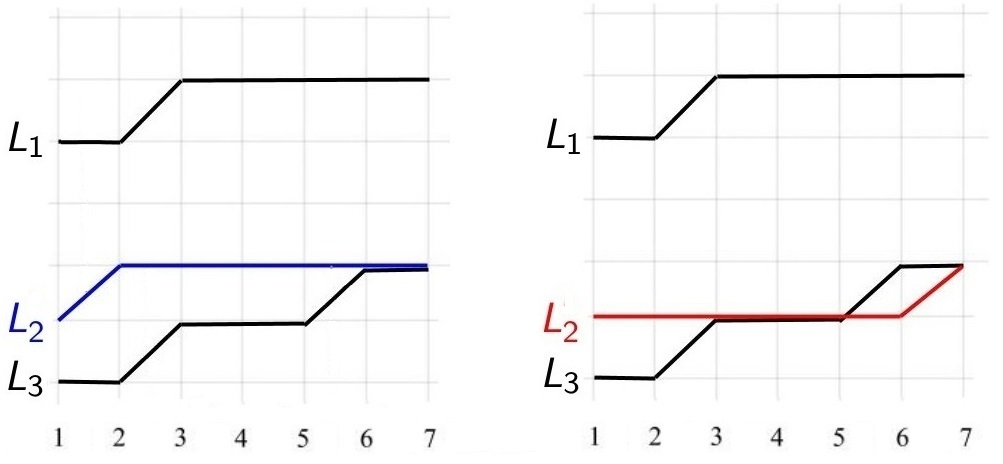
\includegraphics{S3_1.jpg}}
\caption{Two samples of $\{1,2,3\}$-indexed Bernoulli line ensembles with $T_0 = 1$ and $T_1 = 7$. }
\label{S3_1}
\end{figure}
We will often slightly abuse notation and write $\mathfrak{L}: \Sigma \times \llbracket T_0, T_1 \rrbracket \rightarrow \mathbb{Z}$, even though it is not $\mathfrak{L}$ which is such a function, but rather $\mathfrak{L}(\omega)$ for each $\omega \in \Omega$. Furthermore we write $L_i = (\mathfrak{L}(\omega)) (i, \cdot)$ for the index $i \in \Sigma$ path. If $L$ is an up-right path on $\llbracket T_0, T_1 \rrbracket$ and $a, b \in \llbracket T_0, T_1 \rrbracket$ satisfy $a < b$ we let $L\llbracket a, b \rrbracket$ denote the resitrction of $L$ to $\llbracket a,b\rrbracket$. \\

Let $t_i, z_i \in \mathbb{Z}$ for $i = 1,2$ be given such that $t_1 < t_2$ and $0 \leq z_2 - z_1 \leq t_2 - t_1$. We denote by $\Omega(t_1,t_2,z_1,z_2)$ the collection of up-right paths that start from $(t_1,z_1)$ and end at $(t_2,z_2)$, by $\mathbb{P}_{Ber}^{t_1,t_2, z_1, z_2}$ the uniform distribution on $\Omega(t_1,t_2,z_1,z_2)$ and write $\mathbb{E}^{t_1,t_2,z_1,z_2}_{Ber}$ for the expectation with respect to this measure. One thinks of the distribution $\mathbb{P}_{Ber}^{t_1,t_2, z_1, z_2}$ as the law of a simple random walk with i.i.d. Bernoulli increments with parameter $p \in (0,1)$ that starts from $z_1$ at time $t_1$ and is conditioned to end in $z_2$ at time $t_2$ -- this interpretation does not depend on the choice of $p \in (0,1)$. Notice that by our assumptions on the parameters the state space $\Omega(t_1,t_2,z_1,z_2)$ is non-empty.  

Given $k \in \mathbb{N}$, $T_0, T_1 \in \mathbb{Z}$ with $T_0 < T_1$ and $\vec{x}, \vec{y} \in \mathbb{Z}^k$ we let $\mathbb{P}^{T_0,T_1, \vec{x},\vec{y}}_{Ber}$ denote the law of $k$ independent Bernoulli bridges $\{B_i: \llbracket T_0, T_1 \rrbracket  \rightarrow \mathbb{Z} \}_{i = 1}^k$ from $B_i(T_0) = x_i$ to $B_i(T_1) = y_i$. Equivalently, this is just $k$ independent random up-right paths $B_i \in \Omega(T_0,T_1,x_i,y_i)$ for $i = 1, \dots, k$ that are uniformly distributed. This measure is well-defined provided that $\Omega(T_0,T_1,x_i,y_i)$ are non-empty for $i = 1, \dots, k$, which holds if $T_1 - T_0 \geq y_i - x_i \geq 0$ for all $i = 1, \dots, k$. 



The following definition introduces the notion of an $(f,g)$-avoiding Bernoulli line ensemble, which in simple terms is a collection of $k$ independent Bernoulli bridges, conditioned on not-crossing each other and staying above the graph of $g$ and below the graph of $f$ for two functions $f$ and $g$.
\begin{definition}\label{DefAvoidingLawBer}
Let $k \in \mathbb{N}$ and $\mathfrak{W}_k$ denote the set of signatures of length $k$, i.e.
$$\mathfrak{W}_k = \{ \vec{x} = (x_1, \dots, x_k) \in \mathbb{Z}^k: x_1 \geq  x_2 \geq  \cdots \geq  x_k \}.$$
Let $\vec{x}, \vec{y} \in \mathfrak{W}_k$, $T_0, T_1 \in \mathbb{Z}$ with $T_0 < T_1$, and $f: \llbracket T_0, T_1 \rrbracket \rightarrow (-\infty, \infty]$ and $g: \llbracket T_0, T_1 \rrbracket \rightarrow [-\infty, \infty)$ be two functions. 

With the above data we define the {\em $(f,g)$-avoiding Bernoulli line ensemble on the interval $\llbracket T_0, T_1 \rrbracket$ with entrance data $\vec{x}$ and exit data $\vec{y}$} to be the $\Sigma$-indexed Bernoulli line ensemble $\mathfrak{Q}$ with $\Sigma = \llbracket 1, k\rrbracket$ on $\llbracket T_0, T_1 \rrbracket$ and with the law of $\mathfrak{Q}$ equal to $\mathbb{P}^{T_0,T_1, \vec{x},\vec{y}}_{Ber}$ (the law of $k$ independent uniform up-right paths $\{B_i: \llbracket T_0, T_1 \rrbracket \rightarrow \mathbb{R} \}_{i = 1}^k$ from $B_i(T_0) = x_i$ to $B_i(T_1) = y_i$) conditioned on the event 
$$E  = \left\{ f(r) \geq B_1(r) \geq B_2(r) \geq \cdots \geq B_k(r) \geq g(r) \mbox{ for all $r \in \llbracket T_0, T_1 \rrbracket$} \right\}.$$ 
The above definition is well-posed if there exist $B_i \in \Omega(T_0,T_1,x_i,y_i)$ for $i = 1, \dots, k$ that satisfy the conditions in $E$ (i.e. if the set of such up-right paths is not empty). We will denote by $\Omega_{avoid}(T_0, T_1, \vec{x}, \vec{y}, f,g)$ the set of collections of $k$ up-right paths that satisfy the conditions in $E$ and then the distribution on $\mathfrak{Q}$ is simply the uniform measure on $\Omega_{avoid}(T_0, T_1, \vec{x}, \vec{y}, f,g)$. We denote the probability distribution of $\mathfrak{Q}$ as $\mathbb{P}_{avoid, Ber}^{T_0,T_1, \vec{x}, \vec{y}, f, g}$ and write $\mathbb{E}_{avoid, Ber}^{T_0, T_1, \vec{x}, \vec{y}, f, g}$ for the expectation with respect to this measure. When $f=+\infty$ and $g=-\infty$, we simply write $\mathbb{P}^{T_0, T_1, \vec{x},\vec{y}}_{avoid, Ber}$ and $\mathbb{E}^{T_0, T_1, \vec{x},\vec{y}}_{avoid, Ber}$.
\end{definition}

It will be useful to formulate simple conditions under which $\Omega_{avoid}(T_0, T_1, \vec{x}, \vec{y}, f,g)$ is non-empty and thus $\mathbb{P}_{avoid, Ber}^{T_0,T_1, \vec{x}, \vec{y}, f, g}$ well-defined. We accomplish this in the following lemma, whose proof is postponed until Section [Appendix].
\begin{lemma}\label{LemmaWD} Suppose that $k \in \mathbb{N}$ and $T_0, T_1 \in \mathbb{Z}$ with $T_0 < T_1$. Suppose further that $\vec{x}, \vec{y} \in \mathfrak{W}_k$ satisfy $T_1 - T_0 \geq y_i - x_i \geq 0$ for $i = 1, \dots, k$. Suppose further that $f : \llbracket T_0, T_1 \rrbracket \rightarrow (-\infty, \infty]$ and $g : \llbracket T_0, T_1 \rrbracket \rightarrow [-\infty, \infty)$ satisfy $f (i+1) = f(i)$ or $f(i+1) = f(i) + 1$, and $g(i+1) = g(i)$ or $g(i+1) = g(i) +1$ for $i = T_0, \dots, T_1 -1$. Finally, suppose that $f(T_0) \geq x_1, f(T_1) \geq y_1$ and $g(T_0) \leq x_k, g(T_1) \leq y_k$. Then the set $\Omega_{avoid}(T_0, T_1, \vec{x}, \vec{y}, f,g)$ from Definition \ref{DefAvoidingLawBer} is non-empty.
\end{lemma}

The following definition introduces the notion of the Schur Gibbs property, which can be thought of a discrete analogue of the partial Brownian Gibbs property the same way that Bernoulli random walks are discrete analogues of Brownian motion. 
\begin{definition}\label{DefSGP}
Fix a set $\Sigma = \llbracket 1, N \rrbracket$ with $N \in \mathbb{N}$ or $N = \infty$ and $T_0, T_1\in \mathbb{Z}$ with $T_0 < T_1$. A $\Sigma$-indexed Bernoulli line ensemble $\mathfrak{L} : \Sigma \times \llbracket T_0, T_1 \rrbracket \rightarrow \mathbb{Z}$ is said to satisfy the {\em Schur Gibbs property} if it is non-crossing, meaning that 
$$ L_j(i) \geq L_{j+1}(i) \mbox{ for all $j = 1, \dots, N-1$ and $i \in \llbracket T_0, T_1 \rrbracket$},$$
and for any finite $K = \{k_1, k_1 + 1, \dots, k_2 \} \subset \llbracket 1, N - 1 \rrbracket$ and $a,b \in \llbracket T_0, T_1 \rrbracket$ with $a < b$ the following holds.  Suppose that $f, g$ are two up-right paths drawn in $\{ (r,z) \in \mathbb{Z}^2 : a \leq r \leq b\}$ and $\vec{x}, \vec{y} \in \mathfrak{W}_{k_2 - k_1 + 1}$ altogether satisfy that $\mathbb{P}(A) > 0$ where $A$ denotes the event
$$A =\{  ({L}_{k_1}(a), \dots, {L}_{k_2}(a)), \vec{y} = ({L}_{k_1}(b), \dots, {L}_{k_2}(b)), L_{k_1-1} \llbracket a,b \rrbracket = f, L_{k_2+1} \llbracket a,b \rrbracket = g \},$$
where if $k_1 = 1$ we adopt the convention $f = \infty = L_0$. Then for any $\{ B_i \in \Omega(a, b, x_i , y_i) \}_{i = 1}^{k_2 - k_1 +1}$ 
\begin{equation}\label{SchurEq}
\mathbb{P}\left( L_{i + k_1-1}\llbracket a,b \rrbracket = B_{i} \mbox{ for $i = 1, \dots, k_2 - k_1 + 1$} \vert  A \right) = \mathbb{P}_{avoid, Ber}^{T_0,T_1, \vec{x}, \vec{y}, f, g} \left( \cap_{i = 1}^k\{ \mathfrak{Q}_i = B_i \} \right).
\end{equation}
\end{definition}
\begin{remark}\label{RemSGB} In simple words, a Bernoulli line ensemble is said to satisfy the Schur Gibbs property if the distribution of any finite number of consecutive paths, conditioned on their end-points and the paths above and below them is simply the uniform measure on all collection of up-right paths that have the same end-points and do not cross each other or the paths above and below them. 
\end{remark}

\begin{remark}\label{RemSGB2} Observe that in Definition \ref{DefSGP} the index $k_2$ is assumed to be less than or equal to $N-1$, so that if $N < \infty$ the $N$-th path is special and is not conditionally uniform. This is what makes Definition \ref{DefSGP} a discrete analogue of the partial Brownian Gibbs property rather than the usual Brownian Gibbs property. Similarly to the partial Brownian Gibbs propert, see Remark \ref{BGPDeg}, if $N = 1$ then the conditions in Definition \ref{DefSGP} become void. I.e., any Bernoulli line ensemble with one line satisfies the Schur Gibbs property. Also we mention that the well-posedness of $\mathbb{P}_{avoid, Ber}^{T_0,T_1, \vec{x}, \vec{y}, f, g}$ in (\ref{SchurEq}) is a consequence of Lemma \ref{LemmaWD} and our assumption that $\mathbb{P}(A) > 0$.
\end{remark}

\begin{remark} In \cite{CD} the authors studied a generalization of the Gibbs property in Definition \ref{DefSGP} depending on a parameter $t \in (0,1)$, which was called the {\em Hall-Littlewood Gibbs property} due to its connection to Hall-Littlewood polynomials \cite{Mac}. The property in Definition \ref{DefSGP} is the $t \rightarrow 0$ limit of the Hall-Littlewood Gibbs property. Since under this $t \rightarrow 0$ limit Hall-Littlewood polynomials degenerate to Schur polynomials we have decided to call the Gibbs property in Definition \ref{DefSGP} the Schur Gibbs property.
\end{remark}
\begin{remark} \label{restrict}  An immediate consequence of Definition \ref{DefSGP} is that if $M \leq N$, we have that the induced law on $\{L_i\}_{i = 1}^M$ also satisfies the Schur Gibbs property as an $\{1,\dots,M\}$-indexed Bernoulli line ensemble on $\llbracket T_0, T_1 \rrbracket$.
\end{remark}

We end this section with the following definition of the term acceptance probability. 
\begin{definition}\label{DefAP} Assume the same notation as in Definition \ref{DefAvoidingLawBer} and suppose that $ T_1 - T_0 \geq y_i -x_i \geq 0$ for $i =1, \dots, k$. We define the {\em acceptance probability } $Z(  T_0, T_1, \vec{x}, \vec{y}, f, g)$ to be the ratio
\begin{equation}\label{EqAP}
Z(  T_0, T_1, \vec{x}, \vec{y}, f, g) = \frac{|\Omega_{avoid}(T_0, T_1, \vec{x}, \vec{y}, f,g)|}{\prod_{i = 1}^k |\Omega(T_0, T_1, x_i, y_i)|}.
\end{equation}
\end{definition}
\begin{remark}\label{RemAP} The quantity $Z(  T_0, T_1, \vec{x}, \vec{y}, f, g)$ is precisely the probability that if $B_i$ are sampled uniformly from $\Omega(T_0, T_1, x_i, y_i)$ for $i =1 , \dots, k$ then the $B_i$ satisfy the condition
$$ E=  \left\{ f(r) \geq B_1(r) \geq B_2(r) \geq \cdots \geq B_k(r) \geq g(r) \mbox{ for all $r \in \llbracket T_0, T_1 \rrbracket$} \right\}.$$
 Let us explain briefly why we call this quantity an acceptance probability. One way to sample $\mathbb{P}_{avoid, Ber}^{T_0,T_1, \vec{x}, \vec{y}, f, g}$ is as follows. Start by sampling a sequence of i.i.d. up-right paths $B^N_i$ uniformly from $\Omega(T_0, T_1, x_i, y_i)$ for $i =1 , \dots, k$ and $N \in \mathbb{N}$. For each $n$ check if $B^n_1, \dots, B^n_k$ satisfy the condition $E$ and let $M$ denote the smallest index that accomplishes this. If $\Omega_{avoid}(T_0, T_1, \vec{x}, \vec{y}, f,g)$ is non-empty then $M$ is geometrically distributed with parameter $Z(  T_0, T_1, \vec{x}, \vec{y}, f, g)$, and in particular $M$ is finite almost surely and $\{B^M_i\}_{i =1}^k$ has distribution $\mathbb{P}_{avoid, Ber}^{T_0,T_1, \vec{x}, \vec{y}, f, g}$. In this sampling procedure we construct a sequence of candidates $\{B^N_i\}_{i =1}^k$ for $N \in \mathbb{N}$ and reject those that fail to satisfy condition $E$, the first candidate that satisfies it is accepted and has law $\mathbb{P}_{avoid, Ber}^{T_0,T_1, \vec{x}, \vec{y}, f, g}$ and the probability that a candidate is accepted is precisely $Z(  T_0, T_1, \vec{x}, \vec{y}, f, g)$, which is why we call it an acceptance probability.
\end{remark}



%-------------------------------------------------------------------------------------------------------------------------------------------------------------------------------------------------
% Section 2.3
%
%-------------------------------------------------------------------------------------------------------------------------------------------------------------------------------------------------
\subsection{Main result}\label{Section2.3} In this section we present the main result of the paper. We start with the following technical definition.
\begin{definition}\label{Def1} Fix $k \in \mathbb{N}$, $\alpha, \lambda > 0$ and $p \in (0,1)$. Suppose we are given a sequence $\{ T_N \}_{N = 1}^\infty$ with $T_N \in \mathbb{N}$ and that $\{\mathfrak{L}^N\}_{N = 1}^\infty$, $\mathfrak{L}^N = (L^N_1, L^N_2, \dots, L^N_k)$ is a sequence of $\llbracket 1, k \rrbracket$-indexed Bernoulli line ensembles on $ \llbracket -T_N, T_N \rrbracket$. We call the sequence $(\alpha,p,\lambda)$-{\em good} if 
\begin{itemize}
\item for each $N \in \mathbb{N}$ we  have that $\mathfrak{L}^N$ satisfies the Schur Gibbs property of Definition \ref{DefSGP};  
\item there is a function $\psi: \mathbb{N} \rightarrow (0, \infty)$ such that $\lim_{N \rightarrow \infty} \psi(N) = \infty$ and for each $N \in \mathbb{N}$ we have that $ T_N > \psi(N)N^{\alpha}$;
\item  there is a function $\phi: (0, \infty) \rightarrow (0,\infty)$ such that for any $\epsilon > 0$ we have 
\begin{equation}\label{globalParabola}
 \sup_{n \in \mathbb{Z}} \limsup_{N \rightarrow \infty} \mathbb{P} \left( \left|N^{-\alpha/2}(L_1^N(n N^{\alpha}) - p n N^{\alpha} + \lambda n^2 N^{\alpha/2}) \right| \geq \phi(\epsilon) \right) \leq \epsilon.
\end{equation}
\end{itemize}
\end{definition}
\begin{remark} Let us elaborate on the meaning of Definition \ref{Def1}. In order for a sequence of $\mathfrak{L}^N $ of $\llbracket 1, k \rrbracket$-indexed Bernoulli line ensembles on $ \llbracket -T_N, T_N \rrbracket$ to be $(\alpha,p,\lambda)$-{\em good} we want several conditions to be satisfied. Firstly, we want for each $N$ the Bernoulli line ensemble $\mathfrak{L}^N$ to satisfy the Schur Gibbs property. The second condition is that while the interval of definition of $\mathfrak{L}^N$ is finite for each $N$ and given by $\llbracket -T_N, T_N \rrbracket$, we want this interval to grow at least with speed $N^{\alpha}$. This property is quantified by the function $\psi$, which can be essentially thought of as an arbitrary unbounded increasing function on $\mathbb{N}$. The third condition is that we want for each $n \in \mathbb{Z}$ the sequence of random variables $N^{-\alpha/2}(L_1^N(n N^{\alpha}) - p n N^{\alpha})$ to be tight but moreover we want globally these random variables to look like the parabola $-\lambda n^2$. This statement is reflected in (\ref{globalParabola}), which provides a certain uniform tightness of the random variables $N^{-\alpha/2}(L_1^N(n N^{\alpha}) - p n N^{\alpha} + \lambda n^2 N^{\alpha/2}) $. A particular case when (\ref{globalParabola}) is satisfied is for example if we know that  for each $n \in \mathbb{Z}$ the random variables $N^{-\alpha/2}(L_1^N(n N^{\alpha}) - p n N^{\alpha} + \lambda n^2 N^{\alpha/2})$ converge to the same random variable $X$. In the applications that we have in mind these random variables would converge to the $1$-point marginals of the Airy$_2$ process that are all given by the same Tracy-Widom distribution (since the Airy$_2$ process is stationary). Equation (\ref{globalParabola}) is a significant relaxation of the requirement that $N^{-\alpha/2}(L_1^N(n N^{\alpha}) - p n N^{\alpha} + \lambda n^2 N^{\alpha/2})$ all converge weakly to the Tracy-Widom distribution -- the convergence requirement is replaced with a mild but uniform control of all subsequential limits.
\end{remark}

The main result of the paper is as follows.
\begin{theorem}\label{PropTightGood}
Fix $k \in \mathbb{N}$ with $k \geq 2$, $\alpha, \lambda > 0$ and $p \in (0,1)$ and let $\mathfrak{L}^N = (L^N_1, L^N_2, \dots, L^N_k)$ be an $(\alpha, p, \lambda)$-good sequence of $\llbracket 1, k \rrbracket$-indexed Bernoulli line ensembles.  Set
$$f^N_i(s) =  N^{-\alpha/2}(L^N_i(sN^{\alpha}) - p s N^{\alpha} + \lambda s^2 N^{\alpha/2}), \mbox{ for $s\in [-\psi(N) ,\psi(N)]$ and $i = 1,\dots, k -1$,}$$
and extend $f^N_i$ to $\mathbb{R}$ by setting for $i = 1, \dots, k - 1$
$$f^N_i(s) = f^N_i(-\psi(N)) \mbox{ for $s \leq -\psi(N)$ and } f^N_i(s) = f_N(\psi(N)) \mbox{ for $s \geq \psi(N)$}.$$
Let $\mathbb{P}_N$ denote the law of $\{f^N_i\}_{i = 1}^{k-1}$ as a $\llbracket 1, k-1 \rrbracket$-indexed line ensemble (i.e. as a random variable in $(C( \llbracket 1, k -1 \rrbracket \times \mathbb{R}), \mathcal{C})$). Then the sequence $\mathbb{P}_N$ is tight.
\end{theorem}

Roughly, Theorem \ref{PropTightGood} states that if you have a sequence of $\llbracket 1, k \rrbracket$-indexed Bernoulli line ensembles that satisfy the Schur Gibbs property and the top paths of these ensembles under some shift and scaling have tight one-point marginals with a non-trivial parabolic shift, then  under the same shift and scaling the top $k-1$ paths of the line ensemble will be tight. The extension of $f^N_i$ to $\mathbb{R}$ is completely arbitrary and irrelevant for the validity of Theorem \ref{PropTightGood} since the topology on $C( \llbracket 1, k -1 \rrbracket \times \mathbb{R})$ is that of uniform convergence over compacts. Consequently, only the behavior of these functions on compact intervals matters in Theorem \ref{PropTightGood} and not what these functions do near infinity, which is where the modification happens as $\lim_{N \rightarrow \infty} \psi(N) = \infty$  by assumption. The only reason we perform the extension is to embed all Bernoulli line ensembles into the same space $(C( \llbracket 1, k -1 \rrbracket \times \mathbb{R}), \mathcal{C})$.

 We mention that the $k$-th up-right path in the sequence of Bernoulli line ensembles is special and Theorem \ref{PropTightGood} provides no tightness result for it. The reason for this stems from the Schur Gibbs property, see Definition \ref{DefSGP}, which assumes less information for the $k$-th path. In practice, one either has an infinite Bernoulli line ensemble for each $N$ or one has a Bernoulli line ensemble with finite number of paths, which increase with $N$ to infinity. In either of these settings one can use Theorem \ref{PropTightGood} to prove teightness of the full line ensemble - we will have more to say about this in Section [Applications].

The proof of Theorem \ref{PropTightGood} is presented in Section \ref{Section4}. In the next section we derive various properties for Bernoulli line ensembles.







